\setmainfont{Noto Serif}
\setsansfont{Noto Sans}
\setmonofont{Noto Sans Mono}
\setstretch{1.35}

\section{ИК и КР спектроскопии}
1С. Определите полное количество частот $\text{C}-\text{C}$ колебаний для 1,2,3,4-тетра-метилциклобутадиена. Укажите сколько из них можно зарегистрировать с~помощью ИК спектроскопии, а сколько с помощью КР спектроскопии. Сколько из~этих колебаний являются плоскими? Сколько деформационными? Укажите симметрию всех колебаний.
\par
\begin{wrapfigure}{r}{45mm} %this figure will be at the right
    \centering
    \vspace{-1.5ex}
    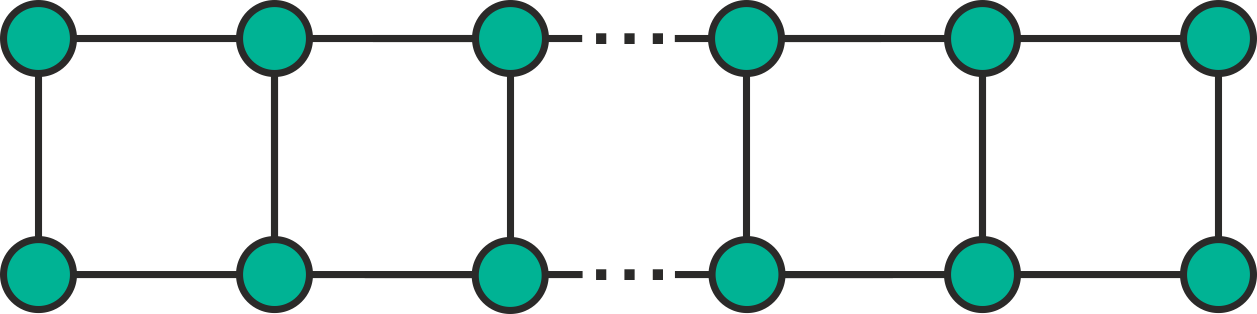
\includegraphics[width=30mm]{images/Fig_2_4_2.png}
    \vspace{-3ex}
\end{wrapfigure}
2C. Определите насколько отличается количество частот колебаний, разрешенных в ИК спектре, от количества частот колебаний, разрешенных в КР спектре, для плоской молекулы из $N$ одинаковых атомов, структура которой схематично изображена на рисунке.
\par
3С. Спектр комбинационного рассеяния карбонат-иона содержит 3 частоты. Используя данный спектр можно ли однозначно установить имеет ли карбонат-ион плоскую или объемную структуру?
\par
\begin{wrapfigure}{r}{58mm} %this figure will be at the right
    \centering
    \vspace{-1mm}
    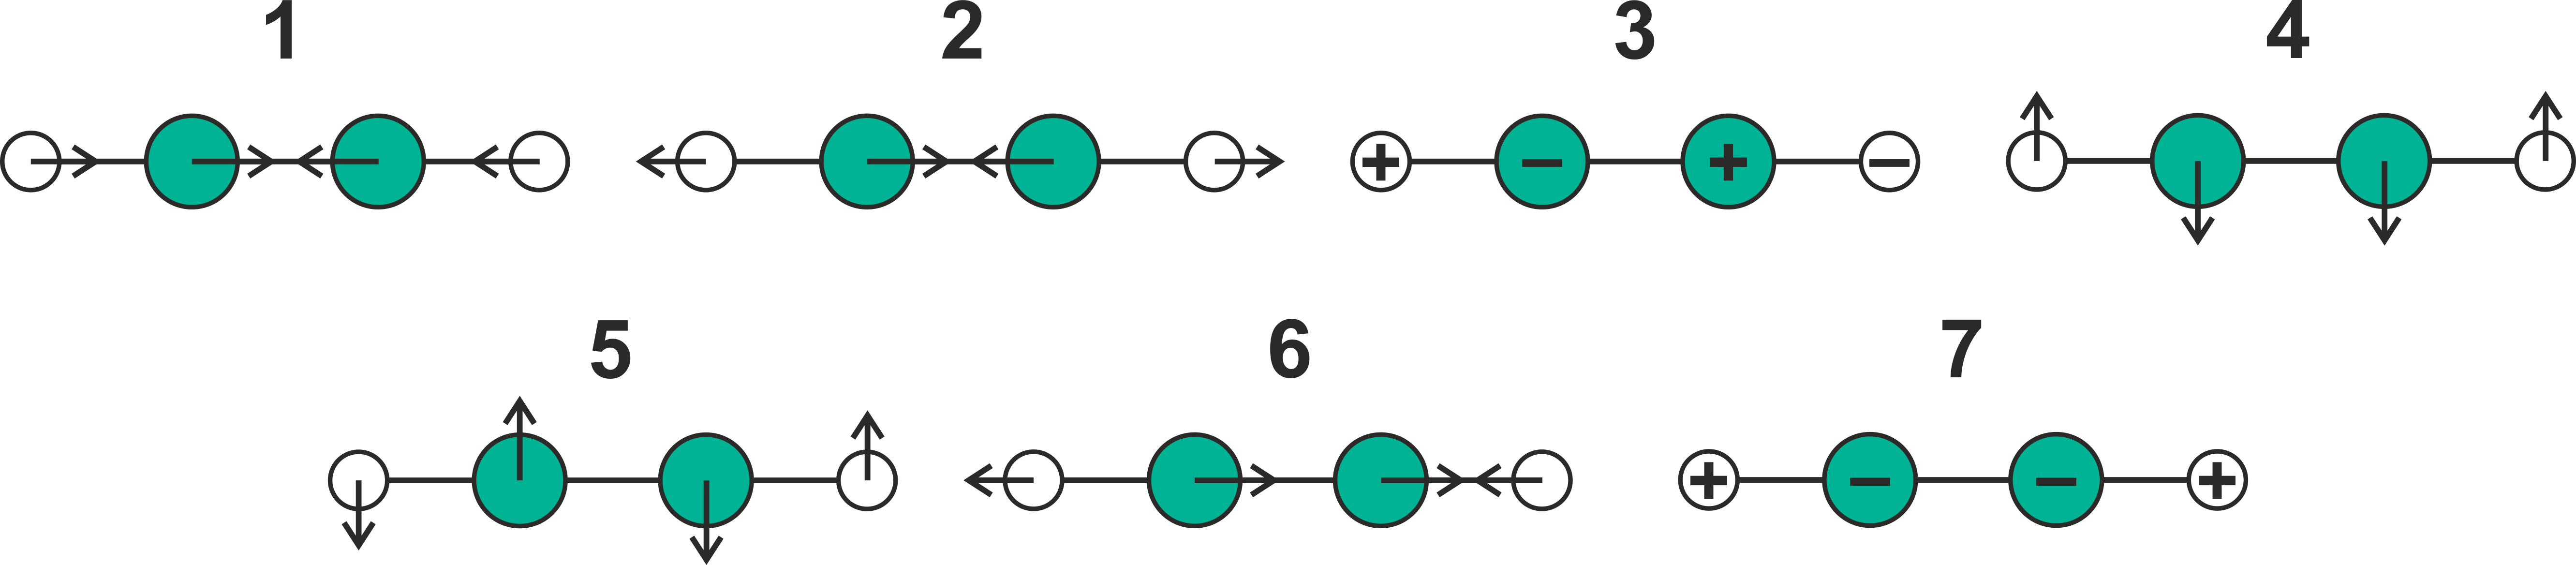
\includegraphics[width=58mm]{images/Fig_2_4_4.png}
    \vspace{-6mm}
\end{wrapfigure}
4К. Какие из изображенных на рисунке колебаний 1–7 молекулы ацетилена можно зарегистрировать с~помощью инфракрасной спектроскопии? Сколько им соответствует частот?
\par
5К. Определите симметрию колебаний цис-изомера плоской нелинейной молекулы $\text{N}_2\text{F}_2$. Какие колебания из найденных проявятся в спектре комбинационного рассеяния?
\par
\begin{wrapfigure}{r}{35mm} %this figure will be at the right
    \centering
    \vspace{-0.7ex}
    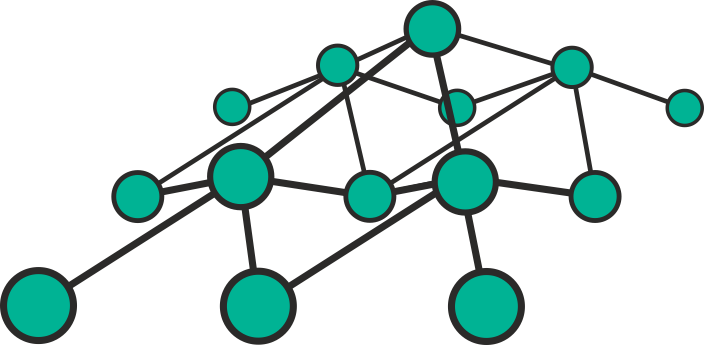
\includegraphics[width=28mm]{images/Fig_2_4_5.png}
    \vspace{-2ex}
\end{wrapfigure}
6C. Определите процент частот, наблюдаемых в ИК спектре, от общего числа частот для молекулы, имеющей строение четырехгранной пирамиды и состоящей из одинаковых атомов, уложенных плотноупакованными слоями как показано на рисунке. В~молекуле всего $N$ слоев, где $N$ – четное число.
\par
7. Какие изменения в количестве частот и их симметрии произойдут в ИК спектре сульфат-иона при его координации к атому металла через атом кислорода?
\par
8С. Можно ли с помощью ИК спектроскопии установить в какой конформации заслоненной или заторможенной находится молекула этана?
\par
9К. При исследовании методом инфракрасной спектроскопии некоторой пробы газообразного углекислого газа был получен спектр, в котором наблюдаются 4 частоты с волновыми числами: 667 и 649 см$^{-1}$, 2349 и 2283 см$^{-1}$. Соотношение интенсивностей в каждой из двух групп линий равно 100 к 1. Определите количество частот, которые должны наблюдаться в ИК спектре углекислого газа, а~также их симметрию. Объясните природу описанного выше экспериментального спектра, в частности природу указанных двух групп линий и относительного положения линий внутри каждой группы. Как будет выглядеть спектр комбинационного рассеяния данной пробы?
\par
10К. Определите число и симметрию валентных и деформационных колебаний в молекуле метана.
\par
11К. Можно ли с помощью ИК спектроскопии различить цис- и транс- изомеры октаэдрического комплекса $[\text{FeCl}_4\text{Br}_2]^{3-}$. 
\par